\PassOptionsToPackage{unicode=true}{hyperref} % options for packages loaded elsewhere
\PassOptionsToPackage{hyphens}{url}
%
\documentclass[9pt,ignorenonframetext,]{beamer}
\usepackage{pgfpages}
\setbeamertemplate{caption}[numbered]
\setbeamertemplate{caption label separator}{: }
\setbeamercolor{caption name}{fg=normal text.fg}
\beamertemplatenavigationsymbolsempty
% Prevent slide breaks in the middle of a paragraph:
\widowpenalties 1 10000
\raggedbottom
\setbeamertemplate{part page}{
\centering
\begin{beamercolorbox}[sep=16pt,center]{part title}
  \usebeamerfont{part title}\insertpart\par
\end{beamercolorbox}
}
\setbeamertemplate{section page}{
\centering
\begin{beamercolorbox}[sep=12pt,center]{part title}
  \usebeamerfont{section title}\insertsection\par
\end{beamercolorbox}
}
\setbeamertemplate{subsection page}{
\centering
\begin{beamercolorbox}[sep=8pt,center]{part title}
  \usebeamerfont{subsection title}\insertsubsection\par
\end{beamercolorbox}
}
\AtBeginPart{
  \frame{\partpage}
}
\AtBeginSection{
  \ifbibliography
  \else
    \frame{\sectionpage}
  \fi
}
\AtBeginSubsection{
  \frame{\subsectionpage}
}
\usepackage{lmodern}
\usepackage{amssymb,amsmath}
\usepackage{ifxetex,ifluatex}
\usepackage{fixltx2e} % provides \textsubscript
\ifnum 0\ifxetex 1\fi\ifluatex 1\fi=0 % if pdftex
  \usepackage[T1]{fontenc}
  \usepackage[utf8]{inputenc}
  \usepackage{textcomp} % provides euro and other symbols
\else % if luatex or xelatex
  \usepackage{unicode-math}
  \defaultfontfeatures{Ligatures=TeX,Scale=MatchLowercase}
\fi
\usetheme[]{Boadilla}
\usecolortheme{beaver}
% use upquote if available, for straight quotes in verbatim environments
\IfFileExists{upquote.sty}{\usepackage{upquote}}{}
% use microtype if available
\IfFileExists{microtype.sty}{%
\usepackage[]{microtype}
\UseMicrotypeSet[protrusion]{basicmath} % disable protrusion for tt fonts
}{}
\IfFileExists{parskip.sty}{%
\usepackage{parskip}
}{% else
\setlength{\parindent}{0pt}
\setlength{\parskip}{6pt plus 2pt minus 1pt}
}
\usepackage{hyperref}
\hypersetup{
            pdftitle={Intro to R - 5. R for Data Science},
            pdfauthor={Michael Hahsler},
            pdfborder={0 0 0},
            breaklinks=true}
\urlstyle{same}  % don't use monospace font for urls
\newif\ifbibliography
\usepackage{color}
\usepackage{fancyvrb}
\newcommand{\VerbBar}{|}
\newcommand{\VERB}{\Verb[commandchars=\\\{\}]}
\DefineVerbatimEnvironment{Highlighting}{Verbatim}{commandchars=\\\{\}}
% Add ',fontsize=\small' for more characters per line
\usepackage{framed}
\definecolor{shadecolor}{RGB}{48,48,48}
\newenvironment{Shaded}{\begin{snugshade}}{\end{snugshade}}
\newcommand{\AlertTok}[1]{\textcolor[rgb]{1.00,0.81,0.69}{#1}}
\newcommand{\AnnotationTok}[1]{\textcolor[rgb]{0.50,0.62,0.50}{\textbf{#1}}}
\newcommand{\AttributeTok}[1]{\textcolor[rgb]{0.80,0.80,0.80}{#1}}
\newcommand{\BaseNTok}[1]{\textcolor[rgb]{0.86,0.64,0.64}{#1}}
\newcommand{\BuiltInTok}[1]{\textcolor[rgb]{0.80,0.80,0.80}{#1}}
\newcommand{\CharTok}[1]{\textcolor[rgb]{0.86,0.64,0.64}{#1}}
\newcommand{\CommentTok}[1]{\textcolor[rgb]{0.50,0.62,0.50}{#1}}
\newcommand{\CommentVarTok}[1]{\textcolor[rgb]{0.50,0.62,0.50}{\textbf{#1}}}
\newcommand{\ConstantTok}[1]{\textcolor[rgb]{0.86,0.64,0.64}{\textbf{#1}}}
\newcommand{\ControlFlowTok}[1]{\textcolor[rgb]{0.94,0.87,0.69}{#1}}
\newcommand{\DataTypeTok}[1]{\textcolor[rgb]{0.87,0.87,0.75}{#1}}
\newcommand{\DecValTok}[1]{\textcolor[rgb]{0.86,0.86,0.80}{#1}}
\newcommand{\DocumentationTok}[1]{\textcolor[rgb]{0.50,0.62,0.50}{#1}}
\newcommand{\ErrorTok}[1]{\textcolor[rgb]{0.76,0.75,0.62}{#1}}
\newcommand{\ExtensionTok}[1]{\textcolor[rgb]{0.80,0.80,0.80}{#1}}
\newcommand{\FloatTok}[1]{\textcolor[rgb]{0.75,0.75,0.82}{#1}}
\newcommand{\FunctionTok}[1]{\textcolor[rgb]{0.94,0.94,0.56}{#1}}
\newcommand{\ImportTok}[1]{\textcolor[rgb]{0.80,0.80,0.80}{#1}}
\newcommand{\InformationTok}[1]{\textcolor[rgb]{0.50,0.62,0.50}{\textbf{#1}}}
\newcommand{\KeywordTok}[1]{\textcolor[rgb]{0.94,0.87,0.69}{#1}}
\newcommand{\NormalTok}[1]{\textcolor[rgb]{0.80,0.80,0.80}{#1}}
\newcommand{\OperatorTok}[1]{\textcolor[rgb]{0.94,0.94,0.82}{#1}}
\newcommand{\OtherTok}[1]{\textcolor[rgb]{0.94,0.94,0.56}{#1}}
\newcommand{\PreprocessorTok}[1]{\textcolor[rgb]{1.00,0.81,0.69}{\textbf{#1}}}
\newcommand{\RegionMarkerTok}[1]{\textcolor[rgb]{0.80,0.80,0.80}{#1}}
\newcommand{\SpecialCharTok}[1]{\textcolor[rgb]{0.86,0.64,0.64}{#1}}
\newcommand{\SpecialStringTok}[1]{\textcolor[rgb]{0.80,0.58,0.58}{#1}}
\newcommand{\StringTok}[1]{\textcolor[rgb]{0.80,0.58,0.58}{#1}}
\newcommand{\VariableTok}[1]{\textcolor[rgb]{0.80,0.80,0.80}{#1}}
\newcommand{\VerbatimStringTok}[1]{\textcolor[rgb]{0.80,0.58,0.58}{#1}}
\newcommand{\WarningTok}[1]{\textcolor[rgb]{0.50,0.62,0.50}{\textbf{#1}}}
\usepackage{longtable,booktabs}
\usepackage{caption}
% These lines are needed to make table captions work with longtable:
\makeatletter
\def\fnum@table{\tablename~\thetable}
\makeatother
\usepackage{graphicx,grffile}
\makeatletter
\def\maxwidth{\ifdim\Gin@nat@width>\linewidth\linewidth\else\Gin@nat@width\fi}
\def\maxheight{\ifdim\Gin@nat@height>\textheight\textheight\else\Gin@nat@height\fi}
\makeatother
% Scale images if necessary, so that they will not overflow the page
% margins by default, and it is still possible to overwrite the defaults
% using explicit options in \includegraphics[width, height, ...]{}
\setkeys{Gin}{width=\maxwidth,height=\maxheight,keepaspectratio}
\setlength{\emergencystretch}{3em}  % prevent overfull lines
\providecommand{\tightlist}{%
  \setlength{\itemsep}{0pt}\setlength{\parskip}{0pt}}
\setcounter{secnumdepth}{0}

% set default figure placement to htbp
\makeatletter
\def\fps@figure{htbp}
\makeatother


% declare overall beamer theme to use as baseline
\usetheme{default}

% make code-output smaller
%\DefineVerbatimEnvironment{Highlighting}{Verbatim}{fontsize=\tiny,commandchars=\\\{\}}

% make console-output smaller:
%\makeatletter
%\def\verbatim{\tiny\@verbatim \frenchspacing\@vobeyspaces \@xverbatim}
%\makeatother

%\setlength{\parskip}{6pt}
%\setlength{\OuterFrameSep}{0pt}

\makeatletter
%\preto{\@verbatim}{\topsep=-2pt \partopsep=-2pt}
\preto{\@verbatim}{\topsep=-\parskip \partopsep=0pt}
\makeatother


\usepackage{multicol}
\newcommand{\btwocol}{\begin{multicols}{2}}
\newcommand{\etwocol}{\end{multicols}}

\title{Intro to R - 5. R for Data Science}
\providecommand{\subtitle}[1]{}
\subtitle{OIT/SMU Libraries Data Science Workshop Series}
\author{Michael Hahsler}
\providecommand{\institute}[1]{}
\institute{OIT, SMU}
\date{}
\titlegraphic{
\includegraphics{WorldChangersRBStackedWebOnlyrgb.png}}

\begin{document}
\frame{\titlepage}

\begin{frame}
\tableofcontents[hideallsubsections]
\end{frame}
\hypertarget{what-is-data-science}{%
\section{What is Data Science?}\label{what-is-data-science}}

\begin{frame}{Data Science}
\protect\hypertarget{data-science}{}

Data Science is still evolving. One definition by Hal Varian (Chief
economist at Google and professor at UC Berkeley) is:

\begin{block}{Data Science}

\emph{The ability to take data -- to be able to understand it, to
process it, to extract value from it, to visualize it, to communicate it
-- that's going to be a hugely important skill in the next decades.} --
Hal Varian

\end{block}

\end{frame}

\begin{frame}{Data Science}
\protect\hypertarget{data-science-2}{}

\begin{figure}
\centering
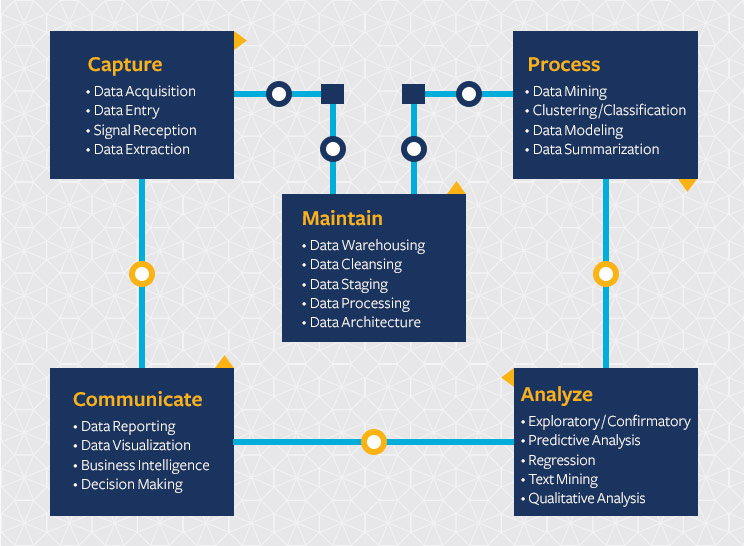
\includegraphics[width=3.64583in,height=\textheight]{figs/DataScienceLifeCycle.jpg}
\caption{Data Science LifeCycle}
\end{figure}

\tiny

Source:
\url{https://datascience.berkeley.edu/about/what-is-data-science/}

\end{frame}

\hypertarget{predictive-modeling}{%
\section{Predictive Modeling}\label{predictive-modeling}}

\begin{frame}{Predictive Modeling}
\protect\hypertarget{predictive-modeling-1}{}

\begin{itemize}
\item
  Data mining
\item
  Machine learning
\item
  Prediction

  \begin{itemize}
  \tightlist
  \item
    regression (predict a number, e.g., the age of a person)
  \item
    classification (predict a label, e.g., yes/no)
  \end{itemize}
\end{itemize}

\end{frame}

\begin{frame}{Predictive Modeling Workflow}
\protect\hypertarget{predictive-modeling-workflow}{}

\begin{figure}
\centering
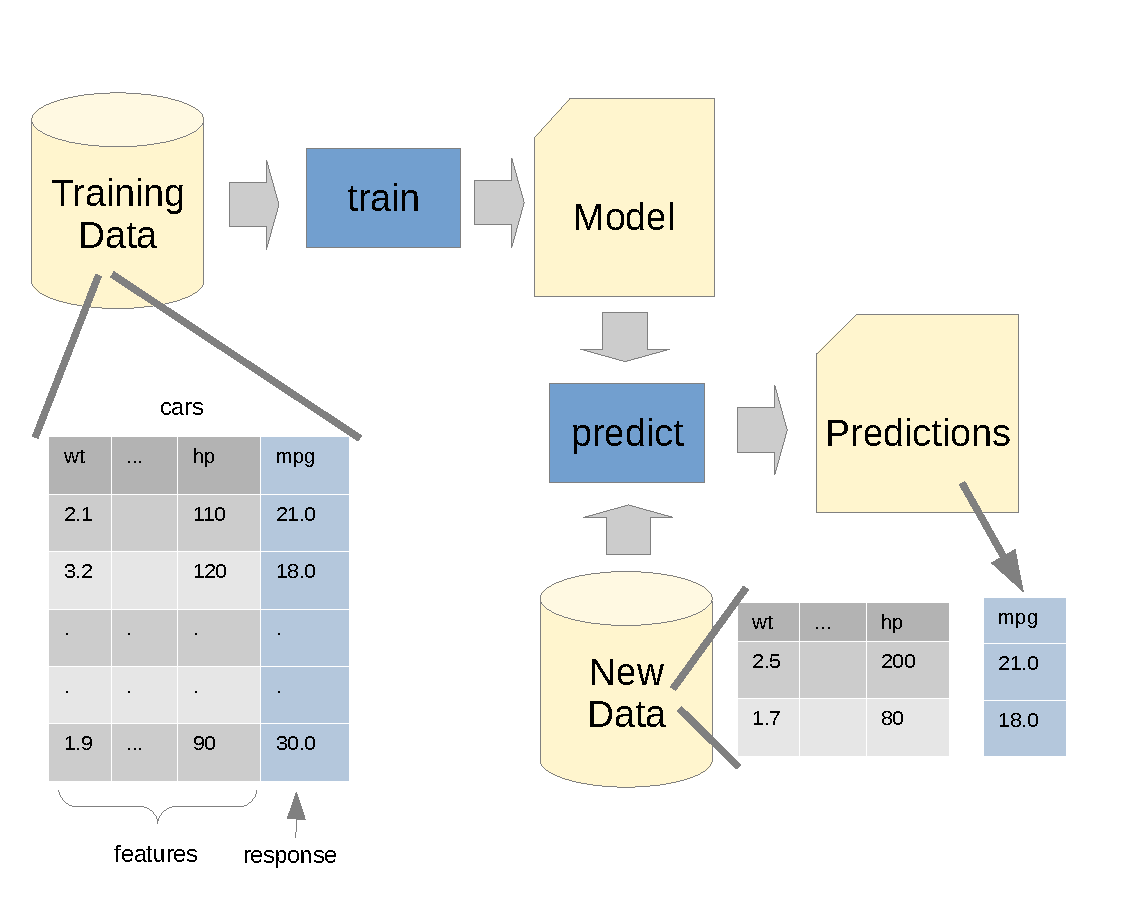
\includegraphics[width=3.64583in,height=\textheight]{figs/pred_model.pdf}
\caption{Workflow of Predictive Modeling}
\end{figure}

\end{frame}

\begin{frame}{Predictive Modeling Workflow in R}
\protect\hypertarget{predictive-modeling-workflow-in-r}{}

\begin{figure}
\centering
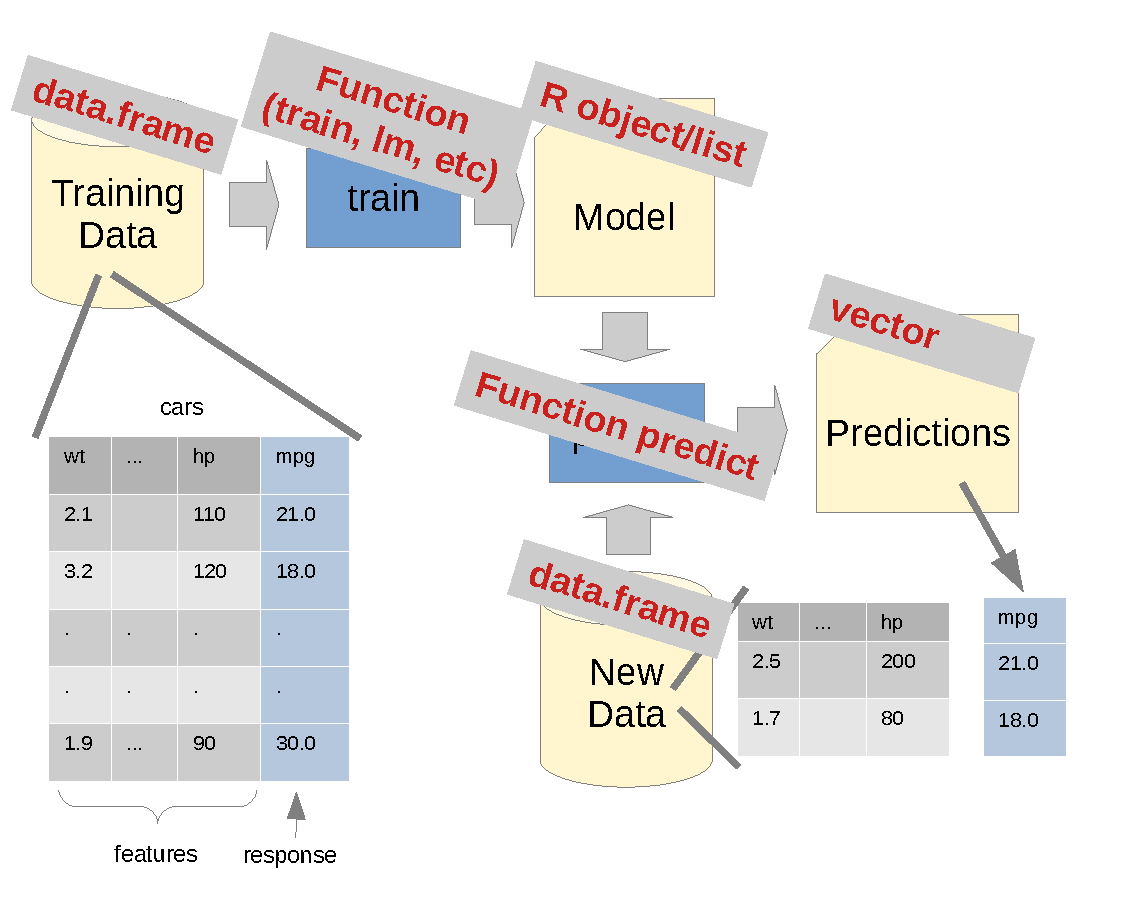
\includegraphics[width=3.64583in,height=\textheight]{figs/pred_model_R.pdf}
\caption{Workflow of Predictive Modeling with R}
\end{figure}

\end{frame}

\begin{frame}[fragile]{Example}
\protect\hypertarget{example}{}

\small

\begin{Shaded}
\begin{Highlighting}[]
\KeywordTok{data}\NormalTok{(mtcars)    }\CommentTok{# Load the dataset}
\NormalTok{knitr}\OperatorTok{::}\KeywordTok{kable}\NormalTok{(}\KeywordTok{head}\NormalTok{(mtcars))}
\end{Highlighting}
\end{Shaded}

\begin{longtable}[]{@{}lrrrrrrrrrrr@{}}
\toprule
& mpg & cyl & disp & hp & drat & wt & qsec & vs & am & gear &
carb\tabularnewline
\midrule
\endhead
Mazda RX4 & 21 & 6 & 160 & 110 & 3.9 & 2.6 & 16 & 0 & 1 & 4 &
4\tabularnewline
Mazda RX4 Wag & 21 & 6 & 160 & 110 & 3.9 & 2.9 & 17 & 0 & 1 & 4 &
4\tabularnewline
Datsun 710 & 23 & 4 & 108 & 93 & 3.9 & 2.3 & 19 & 1 & 1 & 4 &
1\tabularnewline
Hornet 4 Drive & 21 & 6 & 258 & 110 & 3.1 & 3.2 & 19 & 1 & 0 & 3 &
1\tabularnewline
Hornet Sportabout & 19 & 8 & 360 & 175 & 3.1 & 3.4 & 17 & 0 & 0 & 3 &
2\tabularnewline
Valiant & 18 & 6 & 225 & 105 & 2.8 & 3.5 & 20 & 1 & 0 & 3 &
1\tabularnewline
\bottomrule
\end{longtable}

\vfill

\emph{Note}: \texttt{kable} in package \texttt{knitr} is used to
pretty-print the table because the slides were created with Markdown.

\end{frame}

\begin{frame}[fragile]{Example: Predict Miles per Gallon}
\protect\hypertarget{example-predict-miles-per-gallon}{}

\begin{Shaded}
\begin{Highlighting}[]
\KeywordTok{plot}\NormalTok{(mtcars}\OperatorTok{$}\NormalTok{wt, mtcars}\OperatorTok{$}\NormalTok{mpg)}
\end{Highlighting}
\end{Shaded}

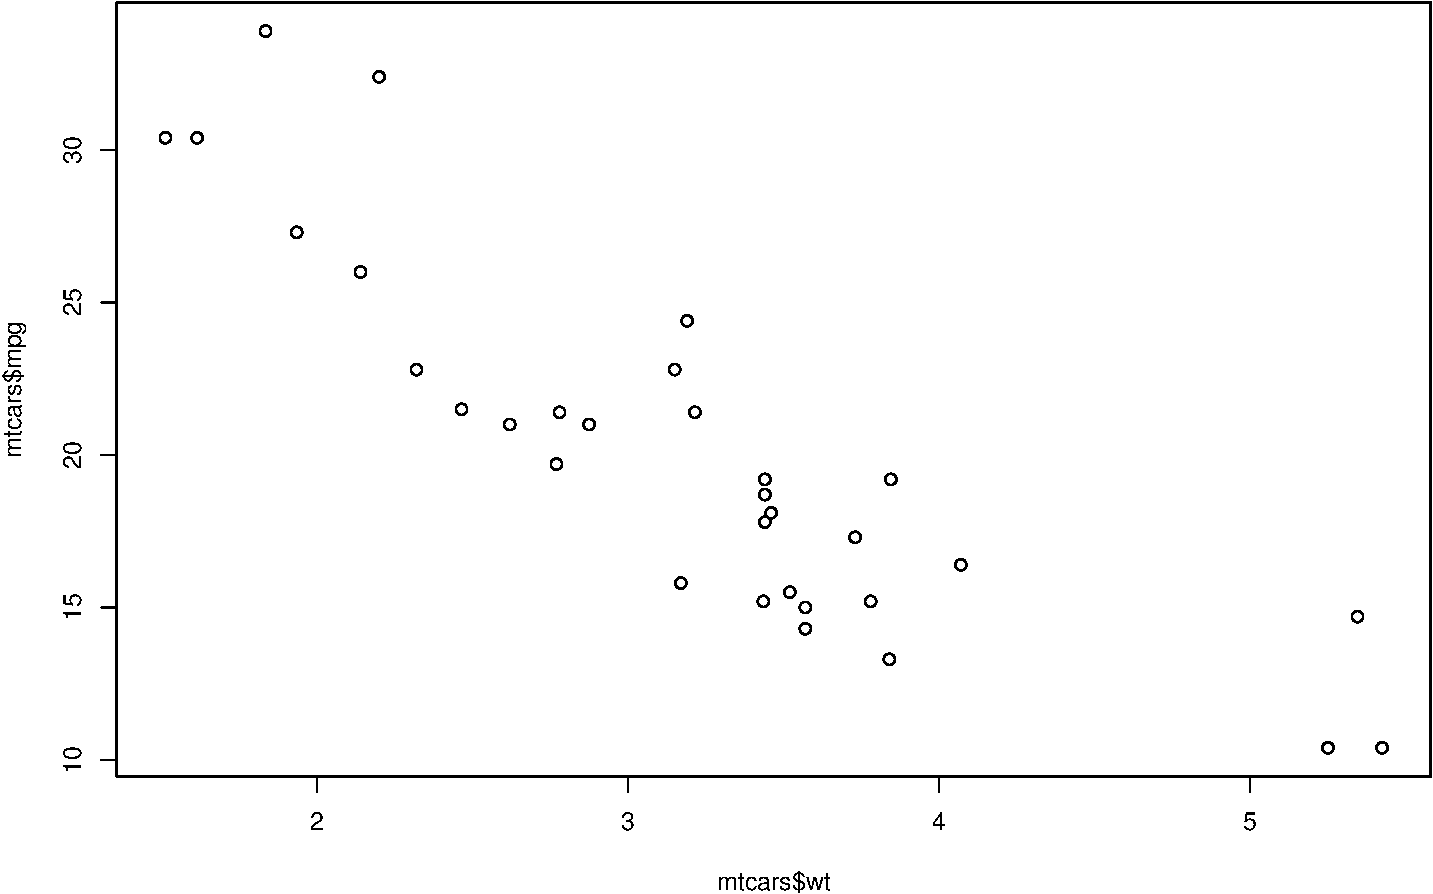
\includegraphics{5_R_for_DataScience_files/figure-beamer/unnamed-chunk-3-1.pdf}

\end{frame}

\begin{frame}[fragile]{Linear Regression}
\protect\hypertarget{linear-regression}{}

\small

\begin{Shaded}
\begin{Highlighting}[]
\NormalTok{model <-}\StringTok{ }\KeywordTok{lm}\NormalTok{(mpg }\OperatorTok{~}\StringTok{ }\NormalTok{wt, }\DataTypeTok{data =}\NormalTok{ mtcars)}
\NormalTok{model}
\end{Highlighting}
\end{Shaded}

\begin{verbatim}
## 
## Call:
## lm(formula = mpg ~ wt, data = mtcars)
## 
## Coefficients:
## (Intercept)           wt  
##       37.29        -5.34
\end{verbatim}

\vfill

\begin{block}{Formula Interface}

R often uses a ``model formula'' to specify models of the from
\texttt{response\ \textasciitilde{}\ predictors}. See
\texttt{?\ formula} for details.

\end{block}

\end{frame}

\begin{frame}[fragile]{Linear Regression: Model summary}
\protect\hypertarget{linear-regression-model-summary}{}

\small

\begin{Shaded}
\begin{Highlighting}[]
\KeywordTok{summary}\NormalTok{(model)}
\end{Highlighting}
\end{Shaded}

\begin{verbatim}
## 
## Call:
## lm(formula = mpg ~ wt, data = mtcars)
## 
## Residuals:
##    Min     1Q Median     3Q    Max 
## -4.543 -2.365 -0.125  1.410  6.873 
## 
## Coefficients:
##             Estimate Std. Error t value Pr(>|t|)    
## (Intercept)   37.285      1.878   19.86  < 2e-16 ***
## wt            -5.344      0.559   -9.56  1.3e-10 ***
## ---
## Signif. codes:  0 '***' 0.001 '**' 0.01 '*' 0.05 '.' 0.1 ' ' 1
## 
## Residual standard error: 3 on 30 degrees of freedom
## Multiple R-squared:  0.753,  Adjusted R-squared:  0.745 
## F-statistic: 91.4 on 1 and 30 DF,  p-value: 1.29e-10
\end{verbatim}

\end{frame}

\begin{frame}[fragile]{Linear Regression: The model as an R object}
\protect\hypertarget{linear-regression-the-model-as-an-r-object}{}

\begin{Shaded}
\begin{Highlighting}[]
\KeywordTok{str}\NormalTok{(model)}
\end{Highlighting}
\end{Shaded}

\begin{verbatim}
## List of 12
##  $ coefficients : Named num [1:2] 37.29 -5.34
##   ..- attr(*, "names")= chr [1:2] "(Intercept)" "wt"
##  $ residuals    : Named num [1:32] -2.28 -0.92 -2.09 1.3 -0.2 ...
##   ..- attr(*, "names")= chr [1:32] "Mazda RX4" "Mazda RX4 Wag" "Datsun 710" "Hornet 4 Drive" ...
##  $ effects      : Named num [1:32] -113.65 -29.116 -1.661 1.631 0.111 ...
##   ..- attr(*, "names")= chr [1:32] "(Intercept)" "wt" "" "" ...
##  $ rank         : int 2
##  $ fitted.values: Named num [1:32] 23.3 21.9 24.9 20.1 18.9 ...
##   ..- attr(*, "names")= chr [1:32] "Mazda RX4" "Mazda RX4 Wag" "Datsun 710" "Hornet 4 Drive" ...
##  $ assign       : int [1:2] 0 1
##  $ qr           :List of 5
##   ..$ qr   : num [1:32, 1:2] -5.657 0.177 0.177 0.177 0.177 ...
##   .. ..- attr(*, "dimnames")=List of 2
##   .. .. ..$ : chr [1:32] "Mazda RX4" "Mazda RX4 Wag" "Datsun 710" "Hornet 4 Drive" ...
##   .. .. ..$ : chr [1:2] "(Intercept)" "wt"
##   .. ..- attr(*, "assign")= int [1:2] 0 1
##   ..$ qraux: num [1:2] 1.18 1.05
##   ..$ pivot: int [1:2] 1 2
##   ..$ tol  : num 1e-07
##   ..$ rank : int 2
##   ..- attr(*, "class")= chr "qr"
##  $ df.residual  : int 30
##  $ xlevels      : Named list()
##  $ call         : language lm(formula = mpg ~ wt, data = mtcars)
##  $ terms        :Classes 'terms', 'formula'  language mpg ~ wt
##   .. ..- attr(*, "variables")= language list(mpg, wt)
##   .. ..- attr(*, "factors")= int [1:2, 1] 0 1
##   .. .. ..- attr(*, "dimnames")=List of 2
##   .. .. .. ..$ : chr [1:2] "mpg" "wt"
##   .. .. .. ..$ : chr "wt"
##   .. ..- attr(*, "term.labels")= chr "wt"
##   .. ..- attr(*, "order")= int 1
##   .. ..- attr(*, "intercept")= int 1
##   .. ..- attr(*, "response")= int 1
##   .. ..- attr(*, ".Environment")=<environment: R_GlobalEnv> 
##   .. ..- attr(*, "predvars")= language list(mpg, wt)
##   .. ..- attr(*, "dataClasses")= Named chr [1:2] "numeric" "numeric"
##   .. .. ..- attr(*, "names")= chr [1:2] "mpg" "wt"
##  $ model        :'data.frame':   32 obs. of  2 variables:
##   ..$ mpg: num [1:32] 21 21 22.8 21.4 18.7 18.1 14.3 24.4 22.8 19.2 ...
##   ..$ wt : num [1:32] 2.62 2.88 2.32 3.21 3.44 ...
##   ..- attr(*, "terms")=Classes 'terms', 'formula'  language mpg ~ wt
##   .. .. ..- attr(*, "variables")= language list(mpg, wt)
##   .. .. ..- attr(*, "factors")= int [1:2, 1] 0 1
##   .. .. .. ..- attr(*, "dimnames")=List of 2
##   .. .. .. .. ..$ : chr [1:2] "mpg" "wt"
##   .. .. .. .. ..$ : chr "wt"
##   .. .. ..- attr(*, "term.labels")= chr "wt"
##   .. .. ..- attr(*, "order")= int 1
##   .. .. ..- attr(*, "intercept")= int 1
##   .. .. ..- attr(*, "response")= int 1
##   .. .. ..- attr(*, ".Environment")=<environment: R_GlobalEnv> 
##   .. .. ..- attr(*, "predvars")= language list(mpg, wt)
##   .. .. ..- attr(*, "dataClasses")= Named chr [1:2] "numeric" "numeric"
##   .. .. .. ..- attr(*, "names")= chr [1:2] "mpg" "wt"
##  - attr(*, "class")= chr "lm"
\end{verbatim}

\end{frame}

\begin{frame}[fragile]{Linear Regression: Plotting the regression line}
\protect\hypertarget{linear-regression-plotting-the-regression-line}{}

\footnotesize

\begin{Shaded}
\begin{Highlighting}[]
\KeywordTok{plot}\NormalTok{(mtcars}\OperatorTok{$}\NormalTok{wt, mtcars}\OperatorTok{$}\NormalTok{mpg)}
\KeywordTok{abline}\NormalTok{(}\KeywordTok{coef}\NormalTok{(model), }\DataTypeTok{col =} \StringTok{"red"}\NormalTok{, }\DataTypeTok{lty =} \DecValTok{2}\NormalTok{, }\DataTypeTok{lwd =} \DecValTok{3}\NormalTok{)}
\end{Highlighting}
\end{Shaded}

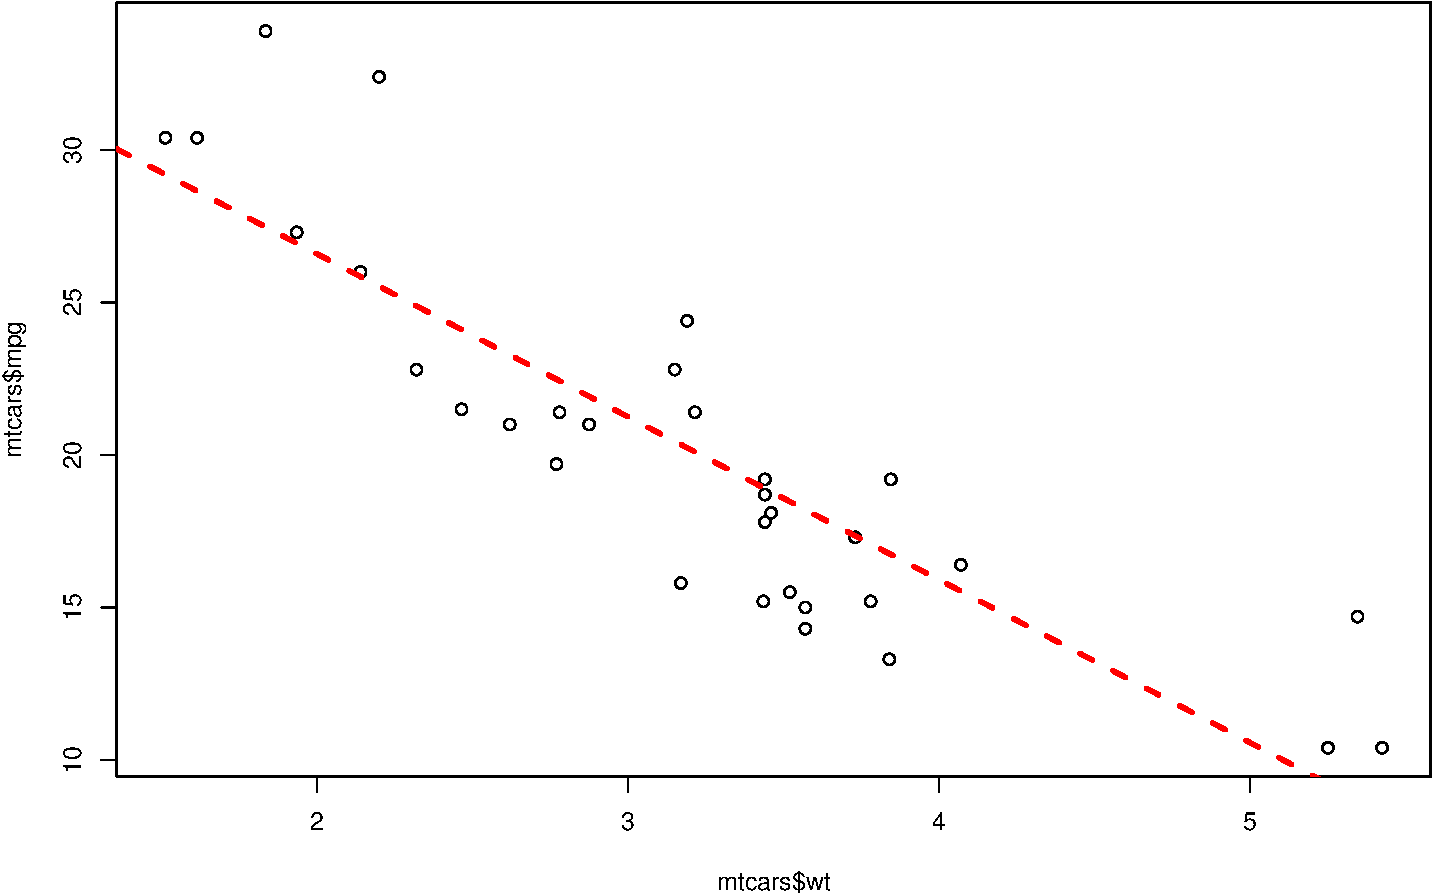
\includegraphics{5_R_for_DataScience_files/figure-beamer/unnamed-chunk-7-1.pdf}

\end{frame}

\begin{frame}[fragile]{Multiple Linear Regression}
\protect\hypertarget{multiple-linear-regression}{}

\footnotesize

\begin{Shaded}
\begin{Highlighting}[]
\NormalTok{model <-}\StringTok{ }\KeywordTok{lm}\NormalTok{(mpg }\OperatorTok{~}\StringTok{ }\NormalTok{wt }\OperatorTok{+}\StringTok{ }\NormalTok{cyl }\OperatorTok{+}\StringTok{ }\NormalTok{hp, }\DataTypeTok{data =}\NormalTok{ mtcars)}
\NormalTok{model}
\end{Highlighting}
\end{Shaded}

\begin{verbatim}
## 
## Call:
## lm(formula = mpg ~ wt + cyl + hp, data = mtcars)
## 
## Coefficients:
## (Intercept)           wt          cyl           hp  
##      38.752       -3.167       -0.942       -0.018
\end{verbatim}

\begin{Shaded}
\begin{Highlighting}[]
\KeywordTok{summary}\NormalTok{(model)}
\end{Highlighting}
\end{Shaded}

\begin{verbatim}
## 
## Call:
## lm(formula = mpg ~ wt + cyl + hp, data = mtcars)
## 
## Residuals:
##    Min     1Q Median     3Q    Max 
## -3.929 -1.560 -0.531  1.185  5.899 
## 
## Coefficients:
##             Estimate Std. Error t value Pr(>|t|)    
## (Intercept)  38.7518     1.7869   21.69   <2e-16 ***
## wt           -3.1670     0.7406   -4.28   0.0002 ***
## cyl          -0.9416     0.5509   -1.71   0.0985 .  
## hp           -0.0180     0.0119   -1.52   0.1400    
## ---
## Signif. codes:  0 '***' 0.001 '**' 0.01 '*' 0.05 '.' 0.1 ' ' 1
## 
## Residual standard error: 2.5 on 28 degrees of freedom
## Multiple R-squared:  0.843,  Adjusted R-squared:  0.826 
## F-statistic: 50.2 on 3 and 28 DF,  p-value: 2.18e-11
\end{verbatim}

\end{frame}

\begin{frame}[fragile]{Prediction}
\protect\hypertarget{prediction}{}

Almost all R models provide a \texttt{predict} function. \vfill

\begin{Shaded}
\begin{Highlighting}[]
\KeywordTok{predict}\NormalTok{(model, }\KeywordTok{head}\NormalTok{(mtcars))}
\end{Highlighting}
\end{Shaded}

\begin{verbatim}
##         Mazda RX4     Mazda RX4 Wag        Datsun 710    Hornet 4 Drive 
##                23                22                26                21 
## Hornet Sportabout           Valiant 
##                17                20
\end{verbatim}

\vfill

\emph{Note:} Prediction is typically done on new or test data. Package
like \texttt{caret} and \texttt{mlr3} and \texttt{Superlearner} help
with this.

\end{frame}

\hypertarget{package-caret}{%
\section{Package Caret}\label{package-caret}}

\begin{frame}[fragile]{Train a model with Caret}
\protect\hypertarget{train-a-model-with-caret}{}

\small

\begin{Shaded}
\begin{Highlighting}[]
\KeywordTok{library}\NormalTok{(}\StringTok{"caret"}\NormalTok{)}
\end{Highlighting}
\end{Shaded}

\begin{verbatim}
## Loading required package: lattice
\end{verbatim}

\begin{verbatim}
## Loading required package: ggplot2
\end{verbatim}

\begin{Shaded}
\begin{Highlighting}[]
\CommentTok{# Simple linear regression model (lm means linear model)}
\NormalTok{model <-}\StringTok{ }\KeywordTok{train}\NormalTok{(mpg }\OperatorTok{~}\StringTok{ }\NormalTok{wt }\OperatorTok{+}\StringTok{ }\NormalTok{cyl }\OperatorTok{+}\StringTok{ }\NormalTok{hp,}
               \DataTypeTok{data =}\NormalTok{ mtcars,}
               \DataTypeTok{method =} \StringTok{"lm"}\NormalTok{)}
\NormalTok{model}
\end{Highlighting}
\end{Shaded}

\begin{verbatim}
## Linear Regression 
## 
## 32 samples
##  3 predictor
## 
## No pre-processing
## Resampling: Bootstrapped (25 reps) 
## Summary of sample sizes: 32, 32, 32, 32, 32, 32, ... 
## Resampling results:
## 
##   RMSE  Rsquared  MAE
##   2.8   0.84      2.3
## 
## Tuning parameter 'intercept' was held constant at a value of TRUE
\end{verbatim}

\end{frame}

\begin{frame}[fragile]{Training a regression tree}
\protect\hypertarget{training-a-regression-tree}{}

\small

\begin{Shaded}
\begin{Highlighting}[]
\CommentTok{# rpart implements CART (here a regression tree)}
\NormalTok{model <-}\StringTok{ }\KeywordTok{train}\NormalTok{(mpg }\OperatorTok{~}\StringTok{ }\NormalTok{wt }\OperatorTok{+}\StringTok{ }\NormalTok{cyl }\OperatorTok{+}\StringTok{ }\NormalTok{hp,}
               \DataTypeTok{data =}\NormalTok{ mtcars,}
               \DataTypeTok{method =} \StringTok{"rpart"}\NormalTok{)}
\end{Highlighting}
\end{Shaded}

\begin{verbatim}
## Warning in nominalTrainWorkflow(x = x, y = y, wts = weights, info =
## trainInfo, : There were missing values in resampled performance measures.
\end{verbatim}

\begin{Shaded}
\begin{Highlighting}[]
\NormalTok{model}
\end{Highlighting}
\end{Shaded}

\begin{verbatim}
## CART 
## 
## 32 samples
##  3 predictor
## 
## No pre-processing
## Resampling: Bootstrapped (25 reps) 
## Summary of sample sizes: 32, 32, 32, 32, 32, 32, ... 
## Resampling results across tuning parameters:
## 
##   cp     RMSE  Rsquared  MAE
##   0.000  4.0   0.55      3.3
##   0.097  4.1   0.54      3.4
##   0.643  5.1   0.48      4.2
## 
## RMSE was used to select the optimal model using the smallest value.
## The final value used for the model was cp = 0.
\end{verbatim}

\end{frame}

\begin{frame}[fragile]{Plotting a regression tree}
\protect\hypertarget{plotting-a-regression-tree}{}

\small

\btwocol

\begin{Shaded}
\begin{Highlighting}[]
\KeywordTok{library}\NormalTok{(rpart.plot)}
\end{Highlighting}
\end{Shaded}

\begin{verbatim}
## Loading required package: rpart
\end{verbatim}

\begin{Shaded}
\begin{Highlighting}[]
\KeywordTok{rpart.plot}\NormalTok{(model}\OperatorTok{$}\NormalTok{finalModel)}
\end{Highlighting}
\end{Shaded}

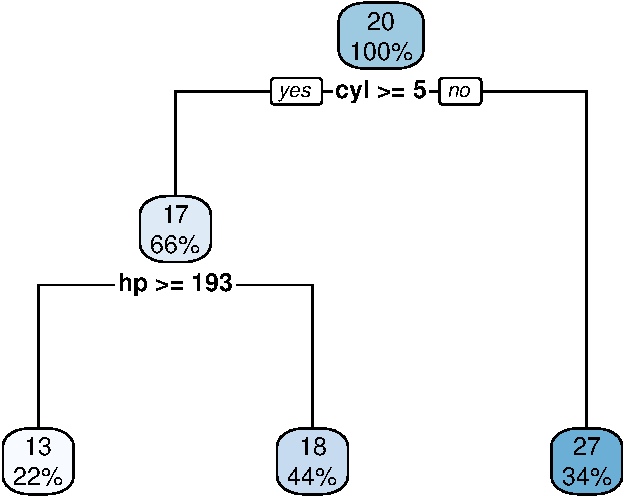
\includegraphics[height=0.5\textheight]{5_R_for_DataScience_files/figure-beamer/unnamed-chunk-12-1}

\begin{Shaded}
\begin{Highlighting}[]
\KeywordTok{varImp}\NormalTok{(model)}
\end{Highlighting}
\end{Shaded}

\begin{verbatim}
## rpart variable importance
## 
##     Overall
## hp    100.0
## cyl    94.6
## wt      0.0
\end{verbatim}

\etwocol

\end{frame}

\hypertarget{exercises}{%
\section{Exercises}\label{exercises}}

\begin{frame}{Exercises}
\protect\hypertarget{exercises-1}{}

\begin{enumerate}
\tightlist
\item
  Load the MLB data set and create a scatter plot of weight by height
  with a regression line added.
\item
  Create a prediction model that predicts weight using position, height,
  and age of the player. Compare different models using caret.
\item
  Create a classification model to predict the position. Decide what
  information is useful for this task.
\end{enumerate}

\end{frame}

\end{document}
